\section{研究背景及研究意义}
\par 近年来,信息技术及人工智能技术已经渗透到我们生活的方方面面,我们幻想的上个世纪许多存在于科幻小说中的内容已经成为现实:如人工智能 AlphaGo 算法击败了人类顶尖的棋手,生产线上大批量的机器人和机械臂取代了人工。
相信不久的将来,大众乘坐宇宙飞船进行星际旅行的梦想将会成为现实。

\par 在制造业领域,工业4.0和智能制造正在产生着新一轮的技术变革。在上海的特斯拉超级工厂,大量的自动化、智能化的设备正在24小时不间断工作,极大地提高了生产效率。
德国的西门子公司也利用工业4.0的理念,将传统的生产线升级为完全自动化、可自主学习的智能生产线。阿里巴巴的“新制造”理念,借助数据和AI技术,打造了一条灵活、智能的供应链,能快速响应市场需求,实现个性化生产。

\par 在众多人工智能领域中,智能机器人无疑是近年来备受关注的领域之一。2021年前11个月,全国有316个机器人项目获得融资,总金额超过330亿人民币。
刚刚过去的北京冬奥会,实现了奥运史上首次利用自动驾驶技术控制无人车的火炬接力、运动员接驳、物资配送(如图\ref{fig:peking}所示)、自动清扫等自动化服务,近百台不同类型的自动驾驶车辆安全有序地运行,既保障了北京冬奥会在复杂天气与疫情的双重挑战下顺利举行,又用实际行动将科技冬奥的主题展现得淋漓尽致。
在我国某大型房地产开发商的建筑工地上\cite{jiqirenjianzhu_chuangxin,jiqirenjianzhu_hulian},上百台不同类别的智能建筑机器人正如火如荼地进行着各项工作。
其中,喷涂机器人可以避免建筑工人在喷涂过程中带来的粉尘职业病和高空作业风险。如图\ref{fig:grinding}所示,地坪研磨机器人可以在建筑物顶层全露天、无遮挡地,进行地面研磨工作,只要用上激光测量,就可以让刮板保持在毫米级的精度,即可以为后续的抛光、铺地板等工作打下高质量的基础,又将建筑工人从这个工地上最辛苦的工作中解放出来。

\begin{figure}[htb]
	\centering
	\begin{minipage}[t]{0.45\linewidth}
		\centering
		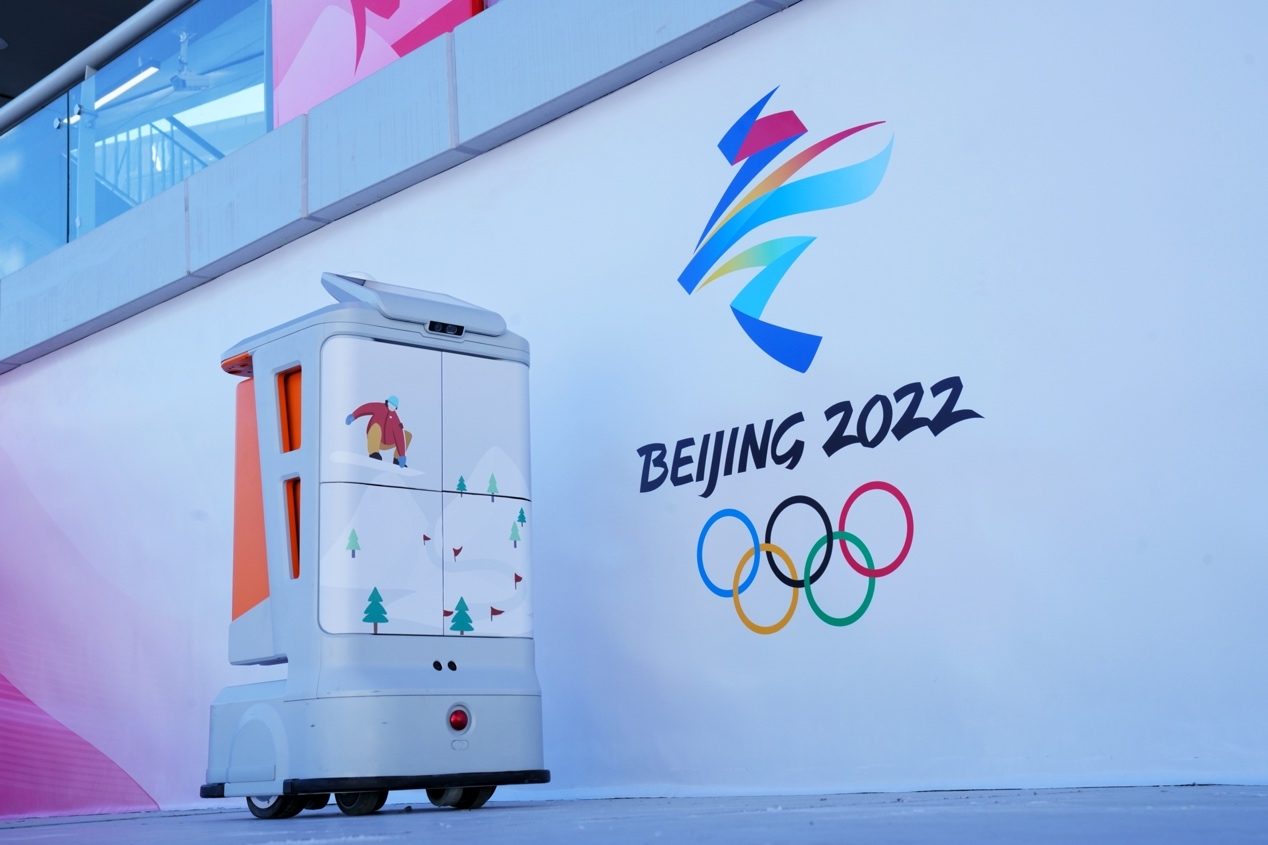
\includegraphics[height=4.5cm,keepaspectratio]{figures/delivery_robot.jpg}
		\caption{北京冬奥会配送机器人}
		\label{fig:peking}
	\end{minipage}
	\begin{minipage}[t]{0.45\linewidth}
		\centering
		\includegraphics[height=4.5cm,keepaspectratio]{figures/floor_grinding_robot.jpg}
		\caption{地坪研磨机器人}
		\label{fig:grinding}
	\end{minipage}
\end{figure}

\par 然而,智能机器人技术仍然面临巨大的挑战及发展空间。在自动驾驶领域,随着技术级别从L2(部分自动驾驶)到L3(有条件的自动驾驶)、L4(高度自动驾驶)级别\cite{unifiedAV}的迈进,其决策系统对感知技术的要求已经不能再局限于二维图像识别和几何模型重建,还需要对周围物体进行实时语义分割,需要在单位时间内处理数量更多、尺寸更大、信息更复杂的全景分割图像\cite{panopticsegmentation,electronics10161960},并实时转换成包含语义信息和实例信息的三维模型。
由于诸多技术的约束,现有的自动驾驶系统只能在天气晴朗、道路交通环境简单的情况下短暂地解放驾驶员的双手\cite{s21165397}。
在上述房地产开发商的建筑工地上,其喷涂机器人只能处理固定的场景,加上机械臂宽度限制和运动时产生的距离误差,每次只能固定在一个地点进行喷涂,然后由人工搬运到另一个地点继续喷涂,不仅使建筑工人消耗大量体力,而且喷涂不够均匀,工作成后仍然需要人工再次修理,产生事倍功半的效果\cite{MANUELDAVILADELGADO2022101787}。

\par 根据上述对智能机器人技术所面临挑战的分析,可以得出结论:如何对重建出的模型进行实时语义分割,是三维重建领域目前面临的关键问题;
如何对动态范围场景进行增量式重建,以及如何提高三维重建及语义分割的速度,快速响应输入的数据,是制约智能机器人大规模应用的重要问题。
这些问题亟需学术及工业界投入大量的人力、资金成本对其进行研究、改进和实践。

\par 针对上述问题,本论文将致力于开发一个基于RGB-D相机的实时三维重建及语义分割系统,输入相机在运动过程中捕获的RGB图像和深度图像,经过预处理后生成相机位姿矩阵和像素级别的语义分割图像,并且利用这些信息对真实世界场景进行实时三维重建及语义分割,转换成包含RGB信息和语义信息的点云模型,并将其重建过程和结果进行可视化展示。

\par 通过使用该实时三维重建及语义分割系统,可以提高智能机器人在各种场景下的适应性和工作效率,为推动智能机器人的广泛应用和产业发展作出贡献。